\documentclass[11pt, a4paper]{article}
\usepackage[english]{babel}
\usepackage[utf8]{inputenc}
\usepackage{amsmath}
\usepackage{multirow}
\usepackage[pdftex]{graphicx}
\usepackage{anysize}
\usepackage{xcolor}
\usepackage{multicol}
\usepackage{hyperref}
\usepackage{float}

\marginsize{1.5cm}{1.5cm}{1.5cm}{1.5cm}

\begin{document}

\sffamily

\title{Adaptation of antibiotic treatment to clinical
practice guidelines in patients aged $\geq65$ years
hospitalised due to community acquired pneumonia}

\author{Fernández Sierra MA$^{1}$, Rueda Domingo MT$^{1}$, Mª del Mar Rodríguez del Águila$^{1}$ et al.\\
\small$^{1}$Medicina Preventiva y Salud Pública. Hospital Universitario Virgen de las Nieves. Granada}

\date{\today}

\maketitle

%\tableofcontents

\begin{abstract}
\url{https://github.com/mmrodri/proyecto_final}

Early, conforming antibiotic treatment in elderly patients hospitalised for community-acquired pneumonia (CAP) is a key factor in the prognosis and mortality. The objective was to examine whether empirical antibiotic treatment was conforming according to the Spanish Society of Pulmonology and Thoracic Surgery guidelines in these patients. Multicentre study in patients aged $\geq65$ years hospitalised due to CAP in the 2013–14 and 2014–15 influenza seasons.We collected socio-demographic information, comorbidities, influenza/pneumococcal vaccination history and antibiotics administered using a questionnaire and medical records. Bivariate analyses and multilevel logistic regression were made. In total, 1857 hospitalised patients were included, 82 of whom required intensive care unit (ICU) admission. Treatment was conforming in 51.4\% (95\% confidence interval (CI) 49.1\%–53.8\%) of patients without ICU admission and was associated with absence of renal failure without haemodialysis (odds ratio (OR) 1.49, 95\% CI 1.15–1.95) and no cognitive dysfunction (OR 1.71, 95\% CI 1.25–2.35), when the effect of the autonomous communitywas controlled for. In patients with ICU admission, treatmentwas conforming in 45.1\% (95\% CI 34.1\%–56.1\%) of patients and was associated with the hospital visits in the last year ($<3$ vs. $\geq3$, OR 2.70, 95\% CI 1.03–7.12) and there was some evidence that this was associated with season. Although the reference guidelines are national, wide variability between autonomous communitieswas found. In patients hospitalised due toCAP, health services should guarantee the administration of antibiotics in a consensual manner that is conforming according to clinical practice guidelines.
\end{abstract}

{\bf Keywords:} Antibiotic treatment; community-acquired pneumonia; correctness; elderly; hospital

\begin{multicols}{2}
\section*{\textcolor{blue}{Introduction}}
The incidence in Europe of community-acquired pneumonia (CAP), one of the main causes of morbidity and mortality in adults, ranges between 1.07 and 1.23 per 1000 persons-year \cite{torres2013risk}, and increases with age (6.2 per 1000 persons-year in persons aged $\geq65$ years and 16.87 per 1000 persons-year in those aged $\geq90$ years) \cite{rivero2016incidence}, leading to a raised hospitalisation rate. CAP is one of the most common reasons for hospitalisation in patients aged $\geq65$ years. Coinciding with Italian data \cite{petrosillo2015treatment}, in Spain there is an increase in hospitalisation according to age group (65–74 years age group 3.94 per 1000, $\geq85$ years age group 25.85 per 1000) \cite{de2017trends}.

Identification of the aetiological agent is essential for conforming treatment, but is often slow and only identifies 50\% of cases \cite{mandell2007infectious}. Therefore, empirical treatment of CAP within the first hours after emergency room admission is recommended. The diagnosis may be guided by the epidemiology of microorganisms in the community and the risk factors of the patients, especially when Pseudomonas aeruginosa infection is suspected in patients with advanced chronic obstructive pulmonary disease (COPD) or generalised bronchiectasis \cite{menendez2010neumonia, gutierrez2005epidemiology}. The pneumococcal and/or influenza vaccination history should also be taken into account, and may have some protective effects \cite{cruzeta2013impact, tomczyk2014use, bennett2012use, centers2010updated, bonten2015polysaccharide, dominguez2010effectiveness} but is not always obtained and, in any case, early empirical treatment is essential.

There is low concordance (6.9\%) between the antibiotic treatment regimens used and those
recommended in international clinical practice guidelines (CPG) \cite{mandell2007infectious, lim2009bts, woodhead2011joint, robinson2014poor}. According to Rossio, in patients aged $\geq65$ years hospitalised and treated empirically, there was conforming treatment according to CPG guidelines \cite{rossio2015adherence} in only 38.8\%.

Successful antimicrobial therapy in CAP is based on patient adherence, which is determined by the treatment duration. Treatments lasting $<7$ days have shown better adherence and, in
addition, the prolonged use of antibiotics is related to a higher frequency of adverse events, prolongs the hospital stay increasing costs, and favours the appearance of micro-organisms multiresistant to available antimicrobials. The Infectious Diseases Society of America/American Thoracic Society consensus guidelines on the management of CAP in adults (IDSA/ATS) [5] and the European Respiratory Society and European Society for Clinical
Microbiology and Infectious Diseases guidelines [15] postulate that the duration of antimicrobial treatment should not be >8 days in patients with a correct response. This was confirmed by a recent multicentre, randomised clinical trial conducted in university
hospitals in Spain \cite{uranga2016duration}.

Studies have compared antibiotic treatment regimens (monotherapy or combined) according to microbiological suspicion and the severity of the patient with pneumonia, documented by
internationally used prognostic scales (Pneumonia Severity Index (PSI) or CURB-65) \cite{eccles2014diagnosis} and 30/90-day mortality \cite{postma2015antibiotic, van2015antibiotics}. The effectiveness of the preferred monotherapy with $\beta$-lactams was not inferior to combination therapy with macrolides or monotherapy with fluoroquinolones.

In Spain, the treatment of patients hospitalised due to CAP normally follows the recommendations of the Spanish Society of Pulmonology and Thoracic Surgery (SEPAR) guidelines \cite{menendez2010neumonia}, which are widely disseminated among specialists in pulmonology, internal medicine and intensive and critical care medicine. The objective of this study was to determine the correctness of empirical antibiotic treatment according to the SEPAR recommendations in patients hospitalised due to CAP.

\section*{\textcolor{blue}{Methods}}
\subsection*{\textcolor{blue}{Study design}}
A multicentre study was carried out in people aged $\geq65$ years hospitalised due to CAP in 20 hospitals in seven Spanish regions (Catalonia, the Basque Country, Castile and Leon, Andalusia, Madrid, Navarra and the Valencian Community) during two influenza seasons (2013–2014 and 2014–2015, October to March both).

\subsection*{\textcolor{blue}{Study population}}
Cases were people aged $\geq65$ years admitted to any of the participating hospitals through the emergency department for $\geq24$ h with a diagnosis of pneumonia whose chest radiograph showed a recent pulmonary infiltrate compatible with pneumonia accompanied by $\geq1$ of the following symptoms: cough, pleural chest pain, dyspnoea, fever or hypothermia in the last 24 h or altered respiratory auscultation not explained by other causes. We excluded institutionalised patients, those with nosocomial pneumonia (onset $\geq2$ days after hospital admission), those residing in another Spanish region and those who did not sign the informed consent.

\subsection*{\textcolor{blue}{Data collection and monitoring}}
All participating hospitals had a teamof health professionals (nurses, physicians) specifically trained to administrate a questionnaire that collected patient information through a personal interview with the patient or a close family member or caregiver when
necessary. Medical records and vaccination cards were reviewed. The questionnaire collected socio-demographic data, comorbidities, history of vaccination against influenza and/or pneumococcus and antibiotics administered during admission.

\subsection*{\textcolor{blue}{Variables of interest}}
The independent variables collected were: autonomous community of hospital, age, sex, history of pneumonia in the last 2 years (yes/no), alcohol consumption (none/sporadic vs. yes), current smoking (non-smoker/smoker/ex-smoker), Barthel index atadmission (scale from 0 to 100 that assesses the level of independence in the basic activities of daily life), influenza season (2013–2014/2014–2015), hospital visits in the last year and primary
care visits in the last year ($<3/\geq3$), mortality during 30 days after hospitalisation, stay days, FINE scale (I–III, IV–V), type of microorganism isolated, comorbidities (diabetes without complications, obesity, renal failure without haemodialysis, congestive
heart disease, disabling neurological disease, seizure disorders and other pulmonary diseases), administration of seasonal influenza and 23-valent pneumococcal polysaccharide vaccines.

Dependent variables were conforming of antibiotic treatment defined according to the regimen administered and according to compliance with the SEPAR \cite{menendez2010neumonia} norm that differentiates patient treatment according to intensive care unit (ICU) admission or not ICU (table~\ref{tab:tabla_tto}) and on the days of hospital stay. In addition, CPGs differentiate treatment according to suspected pneumonia due to P. aeruginosa, and therefore cases with empirical treatment against this microorganism were specifically analysed. Conforming treatment was defined using two variables: the correctness of antibiotic treatment and compliance with the conforming of treatment and treatment duration according to SEPAR guidelines.

\subsection*{\textcolor{blue}{Statistical analysis}}
Descriptive statistics were described using means and standard deviation (S.D.). The bivariate analysis was applied to qualitative variables in the comparison between patients with and without conforming of antibiotic treatment using the $\chi^{2}$ test, the odds ratio (OR) and 95\% confidence intervals (CI). To control the effect of possible variations in patient care between autonomous communities, a forward generalised linear model was used, taking the patient as the first level and the autonomous community as the second level. Two modelswere applied, one with the random effect of the autonomous communities and another including patient variables (fixed effects). The analysis was made using IBM SPSS 19.0 and R
software. A value of $p< 0.05$ was considered statistically significant.

\subsection*{\textcolor{blue}{Ethical considerations}}
The study was approved by the ethics committees of the participating hospitals and the confidentiality of patient information was preserved through the use of identification codes.
\end{multicols}

\begin{figure}[hbt!]
\begin{center}
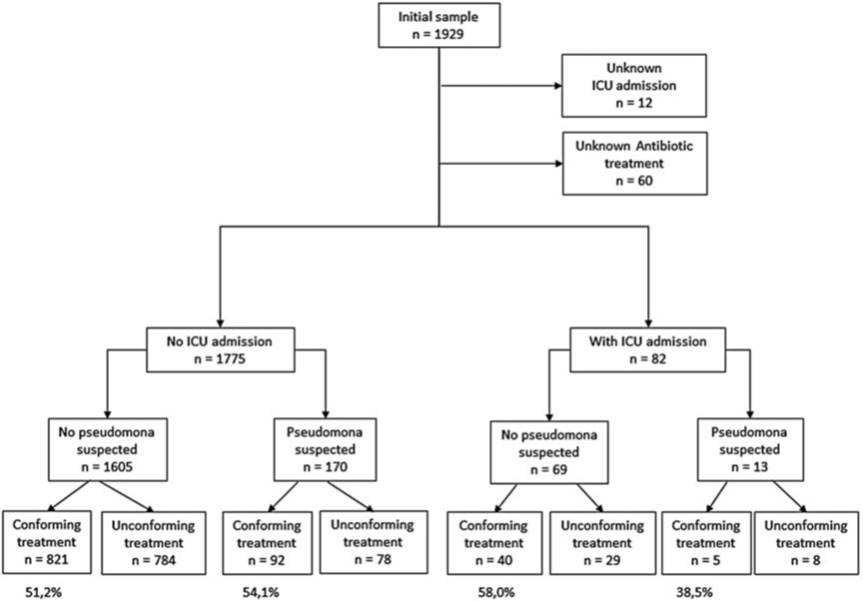
\includegraphics[scale=.7]{algoritmo_casos.jpg}
\caption{\footnotesize Algorithm of the classification of hospitalised cases of pneumonia and percentage of adequacy of antibiotic treatment (at the foot of the figure).}
\label{fig:algoritmo}
\end{center}
\end{figure}

\begin{table}[hbt!]
\centering
\scalebox{0.68}
{
\begin{tabular}{lllllll}
\cline{1-5}
\multirow{2}{*}{}
& \multicolumn{2}{c}{No ICU admission}                                                    & \multicolumn{2}{c}{ICU admission}
&  &  \\ \cline{2-5}
& \multicolumn{1}{c}{Treatment}
& Duration
& \multicolumn{1}{c}{Treatment}
& Duration
&  &  \\ \cline{1-5}
\multirow{2}{*}{\begin{tabular}[c]{@{}l@{}}Conforming treatment\\ without suspicion of\\ pseudomonas\end{tabular}}
& \begin{tabular}[c]{@{}l@{}}Levofloxacin only\\ or moxifloxacin only\end{tabular}
& 7-10 days
& \begin{tabular}[c]{@{}l@{}}Cefotaxime, ceftriaxone or\\ ampilicil-sulbactan+macrolide\end{tabular}
& 7-14 days both treatments
&  &  \\ \cline{2-5}
& \begin{tabular}[c]{@{}l@{}}Third-generation cephalosporins or\\ amoxicillin-clavulanic+macrolide\end{tabular}
& \begin{tabular}[c]{@{}l@{}}7-10 days for\\ both treatments\end{tabular}
& \begin{tabular}[c]{@{}l@{}}Cefotaxime, ceftriaxone or\\ ampicillin-sulbactam +\\ levofloxacin\end{tabular}
& 7-14 days both treatments
&  &  \\ \cline{1-5}
\begin{tabular}[c]{@{}l@{}}Conforming treatment\\ with suspicion of\\ pseudomonas\end{tabular}
& \begin{tabular}[c]{@{}l@{}}Piperacillin-tazobactam or cefepime or\\ cabapenem+ciprofloxacin or\\ levofloxacin or\\ aminoglycoside\end{tabular}
& 14 days
& Same regimen
&  &  &  \\ \cline{1-5}
Unconforming treatment
& \begin{tabular}[c]{@{}l@{}}Levofloxacin or moxifloxacin+\\ third-generation cephalosporins\\ Anoxicilin+clavulanic only\\ Other combinations not contemplated\end{tabular}
& & \begin{tabular}[c]{@{}l@{}}Levofloxacin only\\ Third-ganeration cephalosporin only\\ Amoxicilin-clavulanic only\\ Other combinations not conempleted\end{tabular}
& &  &  \\ \cline{1-5}
\end{tabular}
}
\caption{\footnotesize Classification of conforming/unconforming antibiotic treatment in patients with community-acquired pneumonia, according to the antibiotics received,
intensive care unit admission and duration of antibiotic treatment}
\label{tab:tabla_tto}
\end{table}

\begin{multicols}{2}

\section*{\textcolor{blue}{Results}}
A total of 1929 cases of CAP were collected, of which 12 were excluded because the ICU admission status was unknown and 60 because there was no antibiotic treatment. Therefore, 1857 patients were finally analysed, of whom 1775 were hospitalised on the ward and 82 required ICU admission (figure~\ref{fig:algoritmo}). The mean age was $78.6 \pm 7.4$ years, and 39\% were female. Monotherapy with $\beta$-lactams was administered in 3\% of patients, moxifloxacin in 1.8\% and levofloxacin in 26.6\% of the total.

\begin{figure}[H]
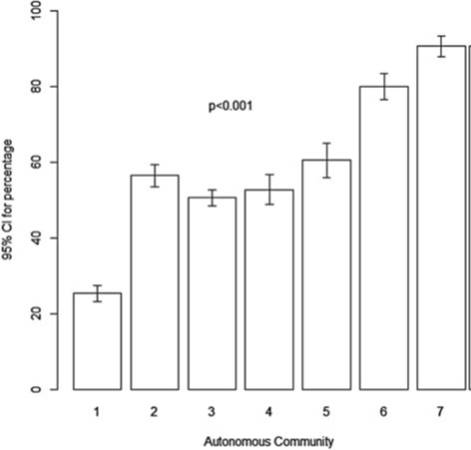
\includegraphics[scale=.60]{adecuacion_ccaa.jpg}
\caption{\footnotesize Percentage of conforming treatment with 95\% confidence interval in hospitalised patients according to autonomous community of residence of the patient.}
\label{fig:ccaa}
\end{figure}

Conforming of antibiotic treatment without taking into account treatment duration was 51.4\% (95\% CI 49.1–53.8) in patients without ICU admission. The variables associated with conforming treatment were COPD (OR 1.24, 95\% CI 1.01–1.52) and absence of renal failure (OR 1.66, 95\% CI 1.30–2.13), congestive heart disease (OR 1.71, 95\% CI 1.39–2.12), haemoglobinopathy or anaemia (OR 1.50, 95\% CI 1.16–1.92), cognitive dysfunction (OR 1.69, 95\% CI 1.27–2.26) and seizure disorders (OR 2.26, 95\% CI 1.06–4.81) (table~\ref{tab:tabla_nouci}). The mean stay was significantly shorter in patients with conforming treatment ($8.89 \pm 8.18$ vs. $11.54 \pm 10.41$, $p < 0.001$), and mortality after 30 days of hospitalisation was worse in patients with uncompliant treatment (OR 1.48, 95\% CI 1.03–2.14). No differences in conforming treatment were found according to the FINE score. Conforming of antibiotic treatment differed according to autonomous community ($p < 0.001$, figure~\ref{fig:ccaa}). The most frequent unconforming treatments in monotherapy (395 patients) were $\beta$-lactamics (96.5\%), and in combination therapy were $\beta$-lactamic + fluoroquinolone with 83.3\%. In both therapies, autonomous communities ranged between 1\% and 42\% of unconforming.

\end{multicols}

\begin{table}[hbt!]
\centering
\scalebox{0.85}
{
\begin{tabular}{lcccc}
\hline
& Conforming treatment & Unconforming treatment & & \\
Variables & ($n=913$) & ($n=862$) & Crude OR & $p$ value \\
\hline
Overall
& 51.4\%
& 48.6\%
& & \\
Barthel index ($\geq40$) 
& 826 (90.5\%)
& 758 (87.9\%) 
& 1.30 (0.96-1.76)
& 0.09 \\
COPD (yes)
& 299 (32.7\%)
& 243 (28.2\%) 
& 1.24 (1.01-1.52)
& 0.037 \\
Renal failure (no)
& 782 (85.7\%)
& 674 (78.2\%)
& 1.66 (1.30-2.13)
& $<0.001$ \\
Disabling neurological disease (no) 
& 842 (92.2\%)
& 781 (90.6\%)
& 1.71 (1.39-2.12)
& $<0.001$ \\
Haemoglobinopaty or anaemia (no)
& 791 (86.6\%) 
& 700 (81.2\%)
& 1.50 (1.16-1.92)
& 0.002 \\
Cognitive dysfunction (no)
& 827 (90.6\%)
& 733 (85.0\%)
& 1.69 (1.27-2.26)
& $<0.001$ \\
Siezure disorders (no)
& 903 (98.9\%)
& 841 (97.6\%)
& 2.26 (1.06-4.81)
& 0.031\\
\hline
\end{tabular}
}
\caption{\footnotesize Significative variables in patients not admitted to the ICU according to conforming of antibiotic treatment}
\label{tab:tabla_nouci}
\end{table}

\begin{multicols}{2}

Of the 82 cases requiring ICU admission, pseudomonas infection was suspected in 13 (15.9\%), according to the type of treatment administered. Treatment compliance with SEPAR guidelines was 58\% in patients without suspicion of P. aeruginosa and 38\% in those with suspicion of pseudomonas infection. Conforming treatment was more frequent in cases collected in the 2013–14 season than those collected in the 2014–15 season (OR 2.60, 95\% CI 1.05–6.44); patients admitted to the ICU with $<3$ hospital visits in the last year had better treatment compliance than those with $\geq3$ hospital visits (OR 3.04, 95\% CI 1.23–7.52) (table~\ref{tab:tabla_uci}).

The multilevel analysis showed similar results between the two models (Table 4). In patients without ICU admission, the variables significantly associated with conforming treatment, taking into account the effect of autonomous communities, were renal failure without haemodialysis (OR 1.49, 95\% CI 1.15–1.95) and cognitive dysfunction (OR 1.71, 95\% CI 1.25–2.35), with a significant trend to significance for COPD (OR 1.23, 95\% CI 0.99–1.54). In patients admitted to the ICU, the variables associated with conforming treatment were $<3$ hospital visits in the last year (OR 2.70, 95\% CI 1.03–7.12), also adjusted by autonomous community. The intraclass correlation coefficient was 22\% for patients without ICU admission and 5\% for those admitted to the ICU.

When considering the treatments administered, taking into account treatment duration, conforming treatment was 26\% (95\% CI 23–28\%) in hospitalised patients and 30\% (95\% CI 18–42\%) in patients admitted to the ICU.

\end{multicols}

\begin{table}[hbt!]
\centering
\scalebox{0.85}
{
\begin{tabular}{lcccc}
\hline
& Conforming treatment & Unconforming treatment & & \\
Variables & ($n=45$) & ($n=37$) & Crude OR & $p$ value \\
\hline
Overall
& 54.9\%
& 45.1\%
& & \\
Influenza season (2013-14) 
& 25 (55.6\%)
& 12 (32.4\%) 
& 2.60 (1.05-6.44)
& 0.04 \\
Hospita visits in last year ($<3$)
& 28 (62.2\%)
& 13 (35.1\%) 
& 3.04 (1.23-7.52)
& 0.02 \\ 
Obesity (yes)
& 13 (28.9\%)
& 5 (13.5\%)
& 2.60 (0.83-8.15)
& 0.09 \\
\hline
\end{tabular}
}
\caption{\footnotesize Significative variables in patients admitted to the ICU according to conforming of antibiotic treatment}
\label{tab:tabla_uci}
\end{table}

\begin{multicols}{2}

\section*{\textcolor{blue}{Discussion}}
The results of this study show that the conforming of empirical treatment according to the SEPAR guidelines in patients aged $\geq65$ years hospitalised due to CAP was greater than that found in European studies (38.8\%) \cite{rossio2015adherence} following the international recommendations of the IDSA/ATS. The international Community-Acquired Pneumonia Organization (CAPO) observational study, using data from hospitalised patients in Venezuela, found a correctness of 55\% \cite{levy2015cumplimiento}, although patients were younger (mean of 54 years).

The comorbidities associated with conforming treatment in patients without ICU admission, after controlling for the effect of autonomous communities, were the absence of renal failure and cognitive dysfunction. This may suggest that, in patients with a history of COPD, physicians provide more conforming empirical antibiotic treatment when the most frequent microorganisms are suspected, and also choose antibiotic regimens that do not require dose adjustment in cases of impaired renal function due to age or associated comorbidities \cite{petrosillo2015treatment}. With respect to the lack of conforming treatment in patients with cognitive impairment, it may be assumed that the information obtained on comorbidities through relatives or caregivers is not sufficiently precise to establish the urgency of antibiotic treatment.

\end{multicols}

\begin{table}[hbt!]
\centering
\scalebox{0.85}
{
\begin{tabular}{lccc}
\hline
& Model 0reatment & Unconforming treatment & & \\
Variables & ($n=45$) & ($n=37$) & Crude OR & $p$ value \\
\hline
Overall
& 54.9\%
& 45.1\%
& & \\
Influenza season (2013-14) 
& 25 (55.6\%)
& 12 (32.4\%) 
& 2.60 (1.05-6.44)
& 0.04 \\
Hospita visits in last year ($<3$)
& 28 (62.2\%)
& 13 (35.1\%) 
& 3.04 (1.23-7.52)
& 0.02 \\ 
Obesity (yes)
& 13 (28.9\%)
& 5 (13.5\%)
& 2.60 (0.83-8.15)
& 0.09 \\
\hline
\end{tabular}
}
\caption{\footnotesize Significative variables in patients admitted to the ICU according to conforming of antibiotic treatment}
\label{tab:tabla_uci}
\end{table}

\begin{table}[hbt!]
\centering
\scalebox{0.85}
{
\begin{tabular}{llcc}
\hline
& {\multirow{2}{*}{Model 0}}
& \multicolumn{2}{c}{Model1}  \\
Fixed effects 
& & OR and 95\% CI 
& p                    \\
COPD (yes)
&  & 1.23 (0.99-1.54)
& 0.060                \\
Renal failure (no)
& & 1.49 (1.15-1.95)
& 0.002                \\
Cognitive dysfunction (no)
& & 1.71 (1.25-2.35)
& $p<0.001$ \\
Randon effects (autonomous community)
& & & \\
Variance (standard error)
& 0.92 (0.9622) & 0.9253 (0.9619)  & \\
Intraclass correlation coefficient
& 21.96\%
& & 
\end{tabular}
\end{table}

\begin{multicols}{2}

In patients admitted to the ICU, conforming treatment was not affected by the comorbidities present at the diagnosis of CAP, but was related to a more stable clinical state in the last year prior to ICU admission or the antibiotic policy in each centre, although there may have been an information bias in the data collection.

The most striking result is that conforming of antibiotic treatment for CAP differs significantly among autonomous communities. Possible reasons might include the adherence of physicians to the SEPAR norms or those of other scientific societies, but we have no information about it. Reasons inherent to the patients themselves, due to their age, multiple pathologies and polypharmacy, as some studies in hospitals \cite{banqueri2014factors} or primary healthcare \cite{fernandez2013appropriateness, perez2002adecuacion} have shown, but these variables have been controlled in our study by statistical models. Likewise, there was a shorter mean stay and lower mortality in the first month after admission in patients with conforming treatment, which has a favourable effect on the efficiency of clinical practice and health outcomes, with diverging results according to other publications \cite{rossio2015adherence, ye2015improvement}.

According to Torres \cite{torres2013guia}, one problem with the norms is that they are drawn up by a maximum of three societies \cite{pachon2009clinical}, making their subsequent implementation in clinical practice difficult. This might justify the variations between autonomous communities in the rates of conforming treatment, which might also be due to the fact that CAP may be treated by medical specialists (pulmonologists or internists) who sometimes follow different therapeutic criteria.

A clinical practice improvement and conforming of antibiotic treatment in NAC could be undertaken by the National Health System (NHS) with a GPC promoving, developed by a multidisciplinary team of health professionals and patients, in which all scientific societies are represented. The GPC Program in the NHS aims to gather opinions of other interest groups that have not participated in it, prior to publication. Dissemination and implementation at national level of this GPC would facilitate the adherence of health professionals to recommendations based on scientific evidence.

The lack of conforming antibiotic treatment might also be due to the fact that persons aged $\geq65$ years have risk factors associated with resistance to antibiotics and, in these patients, treatment must be adapted to these factors for multi-resistant microorganisms. In addition, antimicrobial therapy in the elderly is influenced by physiological changes and comorbidities, with the altered immune function associated with ageing predisposing to suboptimal therapeutic efficacy when antimicrobials are administered. This study could result in actions that increase conforming treatment in this age group.

The initial antibiotic therapy for CAP patients without ICU admission has changed substantially during the last decade \cite{berger2014patterns}, due to the appearance of antibiotic resistance, the evolution of treatment guidelines and initiatives to improve quality that link the financing of care to the guidelines of the health system. In Spain, the quality of health care is considered in the indicators of the NHS and those of the autonomous communities, which include pharmacological prescriptions and conforming of antibiotic treatments that limit the appearance of microbial resistance. Studies have compared their impact on patient mortality and the possible effects on the appearance of resistant bacteria, limiting the use of broad-spectrum antibiotics \cite{postma2015antibiotic, pradelli2015community, wang2016comparative}. The choice of empirical antibiotic treatment for patients with clinical suspicion of CAP admitted to hospital (not the ICU) is complicated by the limited availability of evidence. Some studies have compared empirical treatment strategies of monotherapy with $\beta$-lactam antibiotics vs. combined $\beta$-lactam and macrolide therapy or monotherapy with fluoroquinolone to determine the effect on, which was similar in terms of the length of hospital stay (median 6 days) and 90-day mortality \cite{postma2015antibiotic}. Our study did not investigate mortality but confirmed that the length of hospital stay was associated with conforming of antibiotic treatment.

The strengths of the study include the novelty of identifying patterns of conforming antibiotic treatment in patients admitted due to CAP and the multicentre nature of the study, with the participation of 20 Spanish hospitals. The study had some limitations. First, there was only partial information related to the aetiological aspects of CAP, although it is known that the aetiological agent is determined in $<50\%$ of cases. Second, we did not collect data on antibiotic resistance. Third, we did not collect data on the treating physician that might have influenced the prescribing regime (specialty, age, etc.); however, the PSI was considered as a prognostic scale \cite{menendez2010neumonia} and ICU admission as professional assessment variables, and therefore it may be considered that the aforementioned variables were also considered.

In conclusion, more than half the patients hospitalised due to CAP received conforming empirical antibiotic treatment. After controlling for the effect of the autonomous communities, conforming treatment was only relevant in patients with COPD and no renal failure or cognitive dysfunction. There was a wide variability between autonomous communities without an a priori explanation, since the SEPAR is national in scope. The possible reasons that interfere in adherence to the application of national consensual CPG and which explain the differences found in the correctness of treatment should be studied.

\end{multicols}

\bibliography{bibliog_final.bib}

\bibliographystyle{unsrt}

\end{document}